\documentclass[11pt]{article}
\usepackage[utf8]{inputenc}
\usepackage{amssymb, amsmath, amsthm, changepage, graphicx, caption, subcaption}

\graphicspath{{./images/}}

\title{MAT240 Problem Set 7}
\author{Nicolas Coballe}

\newcommand{\R}{\mathbb{R}}

\newcommand{\N}{\mathbb{N}}

\newcommand{\Z}{\mathbb{Z}}

\newcommand{\F}{\mathbb{F}}

\newcommand{\C}{\mathbb{C}}

\newenvironment{myproof}
{\begin{proof} \begin{adjustwidth}{3em}{0pt}$ $\par\nobreak\ignorespaces}
{\end{adjustwidth} \end{proof}} 

\begin{document}

\maketitle
\begin{flushleft}

1.

$\begin{bmatrix}
1 & 0 \\
0 & 1
\end{bmatrix}$ \\
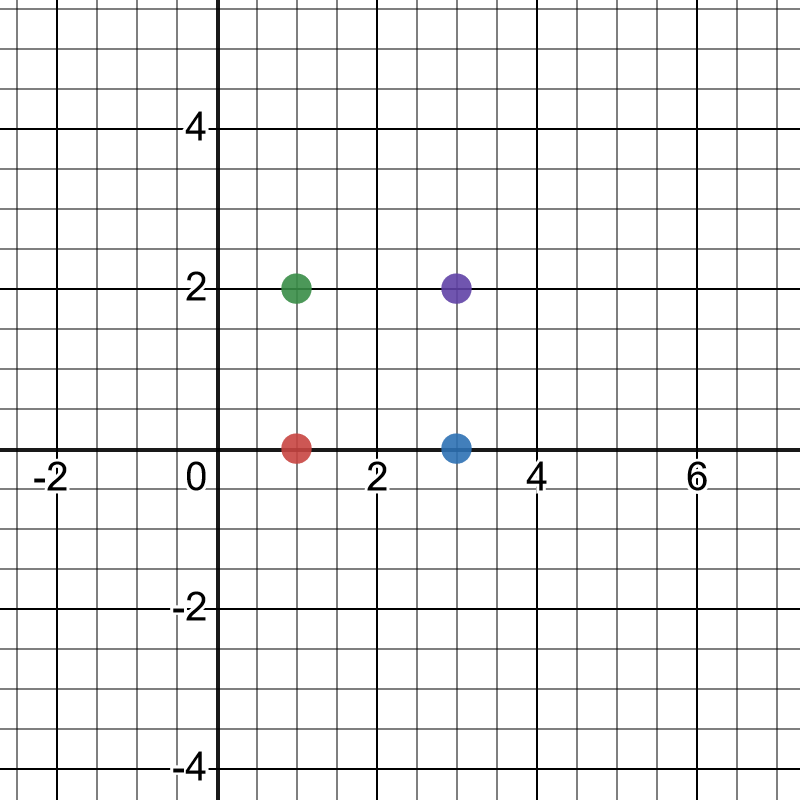
\includegraphics[width=0.3\textwidth]{square1.png} \\

$\begin{bmatrix}
\frac{1}{2} & 0 \\
0 & 2
\end{bmatrix}$ \\
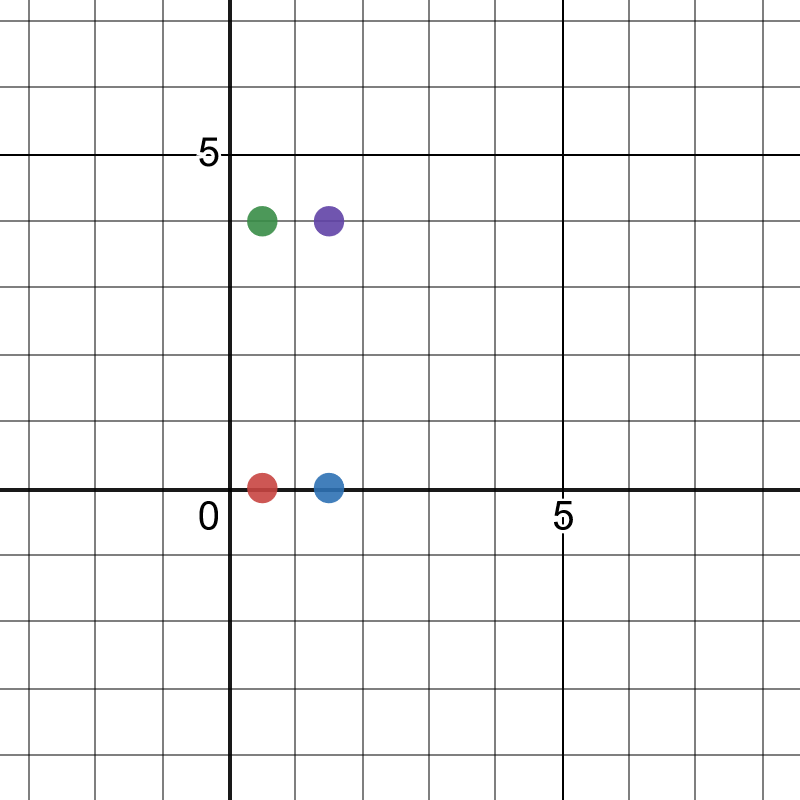
\includegraphics[width=0.3\textwidth]{square2.png} \\

$\begin{bmatrix}
1 & 1 \\
0 & 1
\end{bmatrix}$ \\
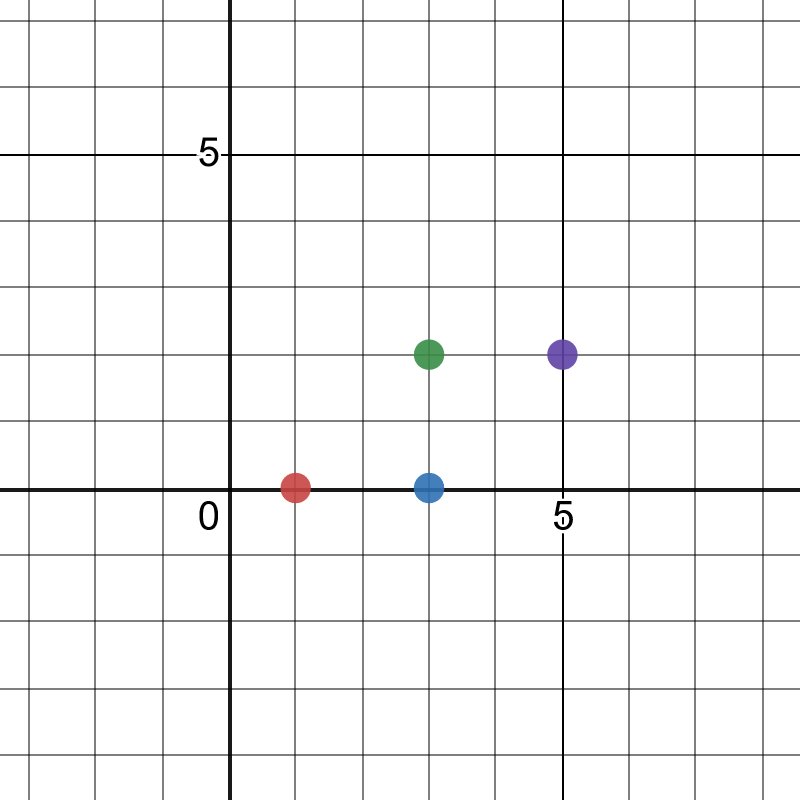
\includegraphics[width=0.3\textwidth]{square3.png} \\

$\begin{bmatrix}
2 & 1 \\
0 & 2
\end{bmatrix}$ \\
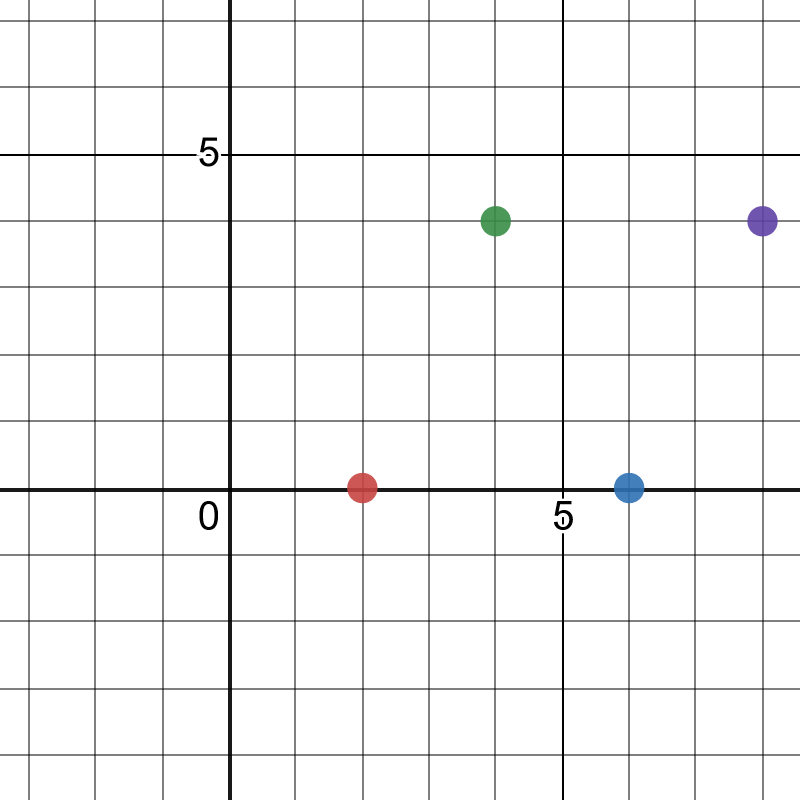
\includegraphics[width=0.3\textwidth]{square4.png} \\

$\frac{1}{\sqrt{2}} \begin{bmatrix}
1 & -1 \\
1 & 1
\end{bmatrix}$ \\
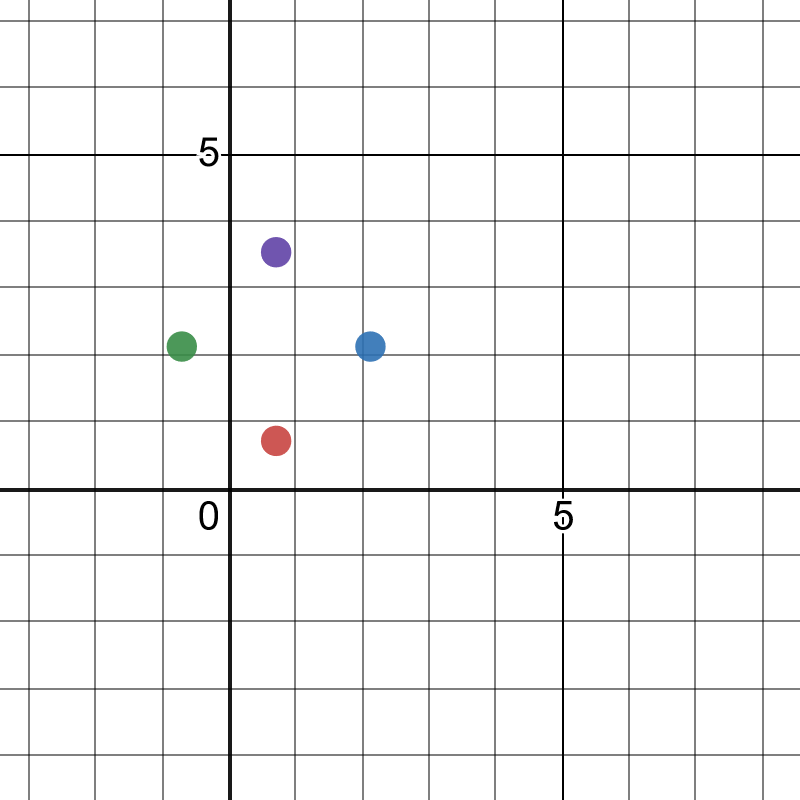
\includegraphics[width=0.3\textwidth]{square5.png} \\

$\frac{1}{2} \begin{bmatrix}
1 & -1 \\
-1 & 1
\end{bmatrix}$ \\
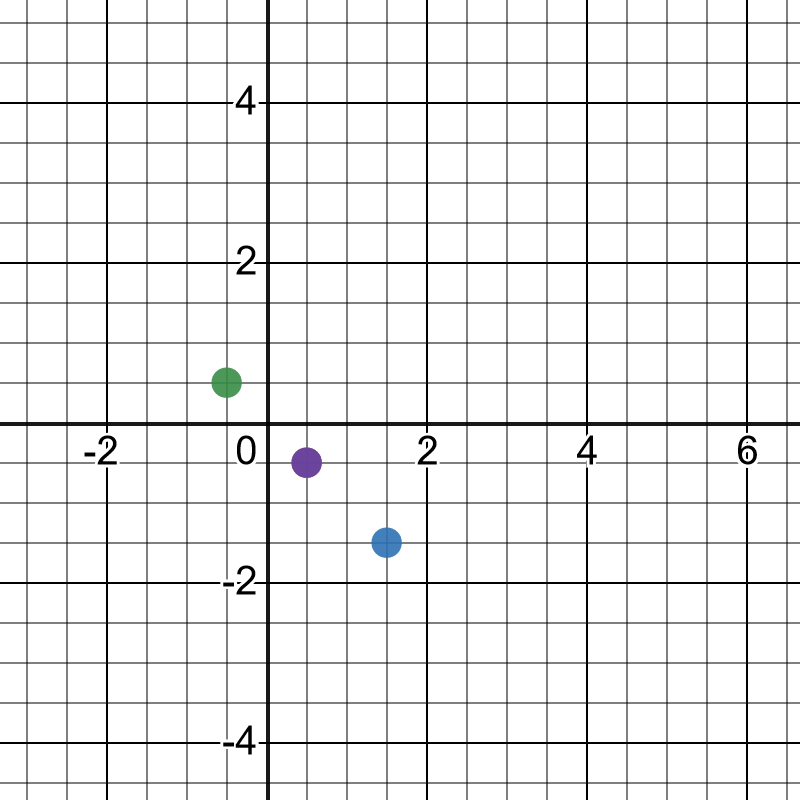
\includegraphics[width=0.3\textwidth]{square6.png} \\

\newpage

2. a)

\begin{myproof}

Consider $f$ is any polynomial in $\mathcal{P}_n(\C)$ with degree $n$. Then, $f$ can be expressed in the form $a_1z + \cdots + a_nz^n, \ a_1,...,a_{n-1} \in \C, a_n \C \setminus \{ 0 \}$. Thus, $f' = 2a_2z + \cdots na_nz^{n-1}$, $f'' = 3 \cdot 2 a_3z + \cdots n(n-1)a_nz^{n-2}$ and etc. Thus it is clear that $f^{(k)}$ is of degree $n-k$ because the highest degree coefficient is never 0; thus, we call the coefficients of $f^{(k)}$ ${a_k}_1,...{a_k}_{n-k} \in \C$. \\
\bigskip

First, we will show that $\beta (f)$ spans $\mathcal{P}_n(\C)$. Consider any polynomial $g \in \mathcal{P}_n(\C)$. $g$ can be expressed as $b_1z + \cdots + b_pz^p, \ b_1,...,b_{p-1} \in \C, b_p \in \C \setminus \{0 \}, 0 \leq p \leq n$. We will show how we can use a linear combination of $\beta (f)$ to create $g$. First, take $\frac{b_p}{{{a_p}_p}}f^{(p)}$. Thus, that will give use some polynomial with $p$-th degree coefficient being equal to $b_p$. We will call $m_0 = \frac{b_p}{{{a_p}_p}}$. Now, we will use a recursive process for each coefficient in $g$ with this first step being our base case: \\
\bigskip
Let $x$ be the $p-i$-th degree coefficient of $m_{0}f^{(p)} + \cdots + m_{i-1}f^{(p-i-1)}$. If $x$ is 0, then we simply add $\frac{b_{p-i}}{{{a_{p-i}}_{p-i}}}f^{(p-i)}$ to $m_0f + \cdots + m_{i-1}f^{(p-i-1)}$ and we call $m_{i} = \frac{b_{p-1}}{{{a_{p-i}}_{p-i}}}$. If $x \neq 0$, then we add $(\frac{-x}{{{a_{p-i}}_{p-i}}} + \frac{b_{p}}{{{a_{p-i}}_{p-i}}})f^{(p-i)}$ to $m_0f + \cdots + m_{i-1}f^{(p-i)}$ and we call $m_{i} = (\frac{-x}{{{a_{p-i}}_{p-i}}} + \frac{b_{p-i}}{{{a_{p-i}}_{p-i}}})$. In either case $m_1f + \cdots + m_{i}f^{(p-i)}$ is now a polynomial which has the same $\ell$-th degree coefficients as $g$ for $p \leq \ell \leq p-i$. If we continue this process $p$ times, we will have a linear combination $m_0f + \cdots + m_pf^{(p)}$ which is equal to $g$ because all the coefficients are equal.\\
\bigskip
Thus, $\beta (f)$ spans $\mathcal{P}_n(\C)$. \\
\bigskip

Now we will show that $\beta (f)$ is linearly independent. We start with the list $f^{(n)}$. Now this list is trivially linearly independent. Consider $f^{(n-1)}$. This has a degree of $1$ which is higher than $f^{(n)}$, which means it isn't in the span of our list. Thus, if we append our list to add $f^{(n-1)}$, our list will still be linearly independent. We know that $f^{(n-i)}$ will be a higher degree than $f^{(n-i+1)}$; thus, $f^{(n-i)}$ is not in the span of $f^{(n)},...,f^{(n-i+1)}$, making $f^{(n)},...,f^{(n-i)}$ linearly independent. Thus if $i = n$, then we have the list $f^{(n)},...,f$, which is the same list as $\beta (f)$ just in a different order, and we also know our new list is linearly independent because the previous list was linearly independent. \\

\bigskip
Thus, $\beta (f)$ is a basis for $\mathcal{P}_n(\C)$.

\end{myproof}

b)

\begin{myproof}

$f(x) = (x-1)^3 = x^3 -3x^2 +3x-1$. Thus $f'(x) = 3x^2 - 6x + 3$, $f''(x) = 6x - 6$, and $f'''(x) = 6$. Thus, the matrix for $_{\beta (f)}I_\alpha$ is as follows:

\begin{align*}
_{\beta (f)}I_\alpha = \begin{bmatrix}
-1 & 3 & -6 & 6 \\
3 & -6 & 6 & 0 \\
-3 & 3 & 0 & 0\\
1 & 0 & 0 & 0
\end{bmatrix}
\end{align*}

The matrix for $_{\alpha}I_{\beta (f)}$ is as follows:

\begin{align*}
_{\alpha}I_{\beta (f)} = \begin{bmatrix}
1 & 0 & 0 & 0 \\
0 & 1 & 0 & 0 \\
0 & 0 & 1 & 0 \\
0 & 0 & 0 & 1
\end{bmatrix}
\end{align*}

\end{myproof}

\newpage

3. a)

\begin{myproof}

Consider matrices $A = [a_{ij}] \in \F^{n \times n}$ and $B = [b_{ij}] \in \F^{n \times n}$. Notice that  the matrix $A + B = [a_{ij} + b_{ij}] \in \F^{n \times n}$ and that the matrix $\lambda A = [ \lambda a_{ij}] \in \F^{n \times n}, \lambda \in \F$. Thus:

\begin{align*}
\text{Tr}(A + B) = & \ \sum_{k = 1}^n a_{kk} + b_{kk} \\
= & \ \sum_{k = 1}^n a_{kk} + \sum_{k = 1}^n b_{kk} \\
= & \ \text{Tr}(A) + \text{Tr}(B) \\
\text{Tr}(\lambda A) = & \ \sum_{k = 1}^n \lambda a_{kk} \\
= & \ \lambda \sum_{k = 1}^n a_{kk} \\
= & \ \lambda \text{Tr}(A)
\end{align*}

Thus, we have shown that the trace of a matrix is linear.

\end{myproof}

b)

\begin{myproof}

Consider the matrices $C = AB = [c_{ij}] \in  \F^{n \times n}$ where $c_{ij} = \sum_{k = 1}^n a_{ik}b_{kj}$ and $D = BA = [d_{ij}] \in  \F^{n \times n}$ where $d_{ij} = \sum_{k = 1}^n b_{ik}a_{kj}$. Consider any index $c_{ii} d_{ii}, \ 1 \leq i \leq n$. $c_{ii} = \sum_{k=1}^n a_{ik}b_{ki}$ and $d_{ii}$ is defined similarly. Then:

\begin{align*}
\text{Tr}(C) = & \sum_{k=1}^n a_{1k}b_{k1} + \cdots + \sum_{k=1}^n a_{1n}b_{n1} \\
\text{Tr}(D) = & \sum_{k=1}^n b_{1k}a_{k1} + \cdots + \sum_{k=1}^n b_{1n}a_{n1}
\end{align*}

Now consider create $n \times n$ matrices $C'$ and $D'$ that consists of the terms in $\text{Tr}(C)$ and $\text{Tr}(D)$ respectfully. Thus:

\begin{align*}
C' =
\begin{bmatrix}
a_{11}b_{11} & \cdots & a_{1n}b_{n1} \\
\vdots & & \vdots \\
a_{n1}b_{1n} & \cdots & a_{nn}b_{nn}
\end{bmatrix} \\
D' =
\begin{bmatrix}
b_{11}a_{11} & \cdots & b_{1n}a_{n1} \\
\vdots & & \vdots \\
b_{n1}a_{1n} & \cdots & b_{nn}a_{nn}
\end{bmatrix}
\end{align*}

Let $N = \{ x \in \N: x \leq n \}$ and define the bijection $f: \N \times \N \rightarrow \N \times \N, \ f(i,j) = (j,i)$. Now notice that $c'_{ij} = a_{ij}b_{ji} = b_{ji}a_{ij} = d'_{ji}$. Thus, because $f$ is a bijection, $D'$ is simply a permuation of $C'$, meaning that $\text{Tr}(C) = \text{Tr}(D)$. Thus, $\text{Tr}(AB) = \text{Tr}(BA)$ as desired.

\end{myproof}

c)

\begin{myproof}

Consider $A = [a_{ij}] \in \F^{n \times n}$ and $B = [b_{ij}] \in \F^{n \times n}$. Then $AB - BA = \begin{bmatrix}
\sum_{k = 1}^n a_{1k}b_{k1} - \sum_{k = 1}^n b_{1k}a_{k1} & \cdots & \sum_{k = 1}^n a_{1k}b_{kn} - \sum_{k = 1}^n b_{1k}a_{kn} \\
\vdots & & \vdots \\
\sum_{k = 1}^n a_{nk}b_{k1} - \sum_{k = 1}^n b_{nk}a_{k1} & \cdots & \sum_{k = 1}^n a_{nk}b_{kn} - \sum_{k = 1}^n b_{nk}a_{kn}
\end{bmatrix}$ \\
\bigskip
Notice that index $(1,1) = a_{11}b_{11} + \cdots + a_{1n}b_{n1} - a_{11}b_{11} - \cdots - a_{n1}b_{1n}$ and $(n,n) =  a_{11}b_{11} + \cdots + a_{1n}b_{n1} - a_{nn}b_{nn} - \cdots - a_{nn}b_{nn}$. Thus, index $(1,1) = -(n,n)$ regardless of our choice of matrices. However, for every other index $(i,j)$, we can choose $A$ and $B$ such that $AB -BA$ has an index that is not always related to another index. This is because consider we want a matrix with one index being 1 and every other index being 0. We can simply take $A$ as the matrix with index 1 in its desired location and $B$ being the identity matrix with one of its 1 being replaced with another non-zero element. Thus $AB-BA$ will be a matrix with 0 everywhere except our desired location. Thus, we can represent the span of $AB-BA$ as a linearly independent list of matrices described using a matrix of matrices $C = [c_{ij}] \in \F^{n \times n}$ where $c_{ij}$ is a $n \times n$ matrix with indexes being 1 at its $(i,j)$ index and 0 everywhere else. However $c_{11} = -c_{nn}$, thus there must be $n^2 -1$ elements in this linearly independent list that spans $AB-BA$. Thus its dimension is $n^2 -1$.

\end{myproof}

d)

\begin{myproof}



\end{myproof}

\newpage

4.

\begin{myproof}

$\begin{bmatrix}
1 & 2 \\
1 & 1 
\end{bmatrix}$ Because the basis vectors are mapped to linearly independent vectors, there is only one way to express the zero vector as linear combination of the transformed basis vectors. Thus, the matrix is injective, and injectivity on a self-map implies surjectivity from \textit{Axler's Linear Algebra Done Right} section 3.69. Dimension of this image is 2 because its a bijection.
\begin{align*}
\begin{bmatrix}
1 & 0 \\
0 & 1
\end{bmatrix}
&\begin{bmatrix}
1 & 2 \\
1 & 1 
\end{bmatrix} \\
\begin{bmatrix}
1 & 0 \\
-1 & 1
\end{bmatrix}
&\begin{bmatrix}
1 & 2 \\
0 & -1 
\end{bmatrix} \\
\begin{bmatrix}
-1 & 2 \\
-1 & 1
\end{bmatrix}
&\begin{bmatrix}
1 & 0 \\
0 & -1 
\end{bmatrix} \\
\begin{bmatrix}
-1 & 2 \\
1 & -1
\end{bmatrix}
&\begin{bmatrix}
1 & 0 \\
0 & 1 
\end{bmatrix} \\
\end{align*}
\bigskip
$\begin{bmatrix}
1 & 2 & 1 \\
1 & 3 & 4 \\
2 & 3 & -1
\end{bmatrix}$
The vector $(5,-3,1)$ is mapped to $5(1,1,2) -3(2,3,3) +(1,4,-1) = 0 $. Thus this map is not injective and not invertible. \\
\bigskip
$ \begin{bmatrix}
1 & 2 & 1 \\
-1 & 1 & 2 \\
1 & 0 & 1
\end{bmatrix}$
The list of vectors $(1,-1,1),(2,1,0),(1,2,1)$ are linearly independent; thus, they are injective, and since the matrix is a self-map, the matrix is invertible.

\begin{align*}
\begin{bmatrix}
1 & 0 & 0 \\
0 & 1 & 0 \\
0 & 0 & 1
\end{bmatrix}
&\begin{bmatrix}
1 & 2 & 1 \\
-1 & 1 & 2 \\
1 & 0 & 1
\end{bmatrix} \\
\begin{bmatrix}
1 & 0 & 0 \\
1 & 1 & 0 \\
-1 & 0 & 1
\end{bmatrix}
&\begin{bmatrix}
1 & 2 & 1 \\
0 & 3 & 3 \\
0 & -2 & 0
\end{bmatrix} \\
\begin{bmatrix}
1 & 0 & 0 \\
-1 & 0 & 1 \\
1 & 1 & 0
\end{bmatrix}
&\begin{bmatrix}
1 & 2 & 1 \\
0 & -2 & 0 \\
0 & 3 & 3
\end{bmatrix} \\
\begin{bmatrix}
0 & 0 & 1 \\
-1 & 0 & 1 \\
1 & 1 & 0
\end{bmatrix}
&\begin{bmatrix}
1 & 0 & 1 \\
0 & -2 & 0 \\
0 & 3 & 3
\end{bmatrix} \\
\begin{bmatrix}
0 & 0 & 1 \\
\frac{1}{2} & 0 & \frac{-1}{2} \\
1 & 1 & 0
\end{bmatrix}
&\begin{bmatrix}
1 & 0 & 1 \\
0 & 1 & 0 \\
0 & 3 & 3
\end{bmatrix} \\
\begin{bmatrix}
0 & 0 & 1 \\
\frac{1}{2} & 0 & \frac{-1}{2} \\
\frac{-1}{2} & 1 & \frac{3}{2}
\end{bmatrix}
&\begin{bmatrix}
1 & 0 & 1 \\
0 & 1 & 0 \\
0 & 0 & 3
\end{bmatrix} \\
\begin{bmatrix}
0 & 0 & 1 \\
\frac{1}{2} & 0 & \frac{-1}{2} \\
\frac{-1}{6} & \frac{1}{3} & \frac{3}{6}
\end{bmatrix}
&\begin{bmatrix}
1 & 0 & 1 \\
0 & 1 & 0 \\
0 & 0 & 1
\end{bmatrix} \\
\begin{bmatrix}
\frac{1}{6} & \frac{-1}{3} & \frac{1}{2} \\
\frac{1}{2} & 0 & \frac{-1}{2} \\
\frac{-1}{6} & \frac{1}{3} & \frac{3}{6}
\end{bmatrix}
&\begin{bmatrix}
1 & 0 & 0 \\
0 & 1 & 0 \\
0 & 0 & 1
\end{bmatrix} \\
\end{align*}
\bigskip
$\begin{bmatrix}
1 & 2 & 1 & 0 \\
2 & 5 & 5 & 1 \\
-2 & -3 & 0 & 3 \\
3 & 4 & -2 & -3
\end{bmatrix}$ The list of vectors $(1,2,-2,3),(2,5,-3,4),(1,5,0,-2),(0,1,3,-3)$ are linearly independent; thus, they are injective, and since the matrix is a self-map, the matrix is invertible. Again, the dimension of the image is 4 because the map is a bijection.
\begin{align*}
\begin{bmatrix}
1 & 0 & 0 & 0 \\
0 & 1 & 0 & 0 \\
0 & 0 & 1 & 0 \\
0 & 0 & 0 & 1
\end{bmatrix}
&\begin{bmatrix}
1 & 2 & 1 & 0 \\
2 & 5 & 5 & 1 \\
-2 & -3 & 0 & 3 \\
3 & 4 & -2 & -3
\end{bmatrix} \\
\begin{bmatrix}
1 & 0 & 0 & 0 \\
-2 & 1 & 0 & 0 \\
2 & 0 & 1 & 0 \\
-3 & 0 & 0 & 1
\end{bmatrix}
&\begin{bmatrix}
1 & 2 & 1 & 0 \\
0 & 1 & 3 & 1 \\
0 & 1 & 2 & 3 \\
0 & -2 & -5 & -3
\end{bmatrix} \\
\begin{bmatrix}
5 & -2 & 0 & 0 \\
-2 & 1 & 0 & 0 \\
4 & -1 & 1 & 0 \\
-7 & -2 & 0 & 1
\end{bmatrix}
&\begin{bmatrix}
1 & 0 & -5 & -2 \\
0 & 1 & 3 & 1 \\
0 & 0 & -1 & 2 \\
0 & 0 & 1 & -1
\end{bmatrix} \\
\begin{bmatrix}
5 & -2 & 0 & 0 \\
-2 & 1 & 0 & 0 \\
-4 & 1 & -1 & 0 \\
-7 & -2 & 0 & 1
\end{bmatrix}
&\begin{bmatrix}
1 & 0 & -5 & -2 \\
0 & 1 & 3 & 1 \\
0 & 0 & 1 & -2 \\
0 & 0 & 1 & -1
\end{bmatrix} \\
\begin{bmatrix}
-15 & 3 & -5 & 0 \\
10 & -2 & 3 & 0 \\
-4 & 1 & -1 & 0 \\
-3 & 1 & 1 & 1
\end{bmatrix}
&\begin{bmatrix}
1 & 0 & 0 & -2 \\
0 & 1 & 0 & 1 \\
0 & 0 & 1 & -2 \\
0 & 0 & 0 & 1
\end{bmatrix} \\
\begin{bmatrix}
-51 & 15 & 7 & 12 \\
31 & -9 & 4 & -7 \\
-10 & 3 & 1 & 2 \\
-3 & 1 & 1 & 1
\end{bmatrix}
&\begin{bmatrix}
1 & 0 & 0 & 0 \\
0 & 1 & 0 & 0 \\
0 & 0 & 1 & 0 \\
0 & 0 & 0 & 1
\end{bmatrix} \\
\end{align*}

\end{myproof}

\newpage

5. 1)

\begin{myproof}

\textbf{Reflexive} \\
$x -x = 0 \in U$, thus $x \sim x$. \\
\bigskip

\textbf{Symmetric} \\
If $x \sim y$, then $x - y \in U$. Due to the existence of additive inverses $-(x-y) \in U$. But $-(x-y) = y - x \in U$. Thus, $y \sim x$. \\
\bigskip

\textbf{Transitive} \\
If $x \sim y$ and $y \sim z$, then $x - y \in U$ and $y - z \in U$. Thus, $x-y + (y-z) \in U$. However, $x-y + (y-z) = x-z \in U$. Thus, $x \sim z$. \\
\bigskip
Thus, $\sim$ is an equivalence relation.

\end{myproof}

2)

\begin{myproof}

Let vector addition be defined as $[v] + [w] = [v+w]$, and let scalar multiplication be defined as $\lambda [v] = [\lambda v]$. Furthermore, the additive identity of $V/U$ is $[0]$, and for any $[v] \in V/U$, the additive inverse of $[v]$ is $[-v]$ because $[v] + [-v] = [v-v] = [0]$. Thus, $V/U$ is a vector space.

\end{myproof}

3)

\begin{myproof}

From the Fundamental Theorem of Linear Maps in \textit{Axler's Linear Algebra Done Right}, $\text{dim} V = \text{dim null}\pi + \text{dim range}\pi$. However, dim null $\pi = U$ because only elements in $U$ can sum to 0, and dim range $\pi= V/U$ because $\pi$ is clearly surjective. Thus, $\text{dim} V = \text{dim}U + \text{dim} V/U$; thus, $\text{dim} V/U = \text{dim}V - \text{dim}U$ as desired.

\end{myproof}

\newpage

6. 1)

\begin{myproof}

Consider $f(u) \in \text{Im}(f), \ u \in U$. By assumption, $(g \circ f)(u) = 0$. Thus $g(f(u)) = 0$ for any arbitrary $u$. Thus $f(u)$ is also in null$(g)$. \\
\bigskip
For an example, take $U = \R, \ V = \R^3, \ W = \R$. Where $f: U \rightarrow V, \ f(x) = (x,0,0)$ and $g: V \rightarrow W, \ g(x,y,z) = z$. Thus, Im$(f) = \{ (x,0,0): x \in \R \}$, which is a proper subspace of Null$(g) = \{ (x,y,0): x,y \in \R \} \subset V$.

\end{myproof}

\begin{myproof}

By the Fundamental Theorem of Linear Maps, $\text{dim} V = \text{dim null} (Q) + \text{dim range} (Q)$. However, $\text{null} (Q) = \text{range} (Q)$. Thus $\text{dim}V = 2 \cdot \text{dim null} (Q)$. Thus, dim$V$ is even. \\
\bigskip
For example, consider $V = \{ 0 \}$ and $Q: V \rightarrow V, \ Q(v) = v$. Thus, Im$(Q) = \text{null}(Q) = \{ 0 \}$. Thus, dim$V = 2 \cdot \text{dim null}(Q)  = 2 \cdot 0 = 0$, which is even.

\end{myproof}

\newpage

10. 1)

\begin{align*}
\begin{bmatrix}
0 & 1 & -1 & 0 & 0 & 0 \\
1 & 0 & 0 & -1 & 0 & 0 \\
0 & -1 & 0 & 0 & -1 & 0 \\
-1 & 0 & 0 & 0 & 0 & -1 \\
0 & 0 & 1 & 1 & 1 & 1
\end{bmatrix}
\end{align*}


2)

The rank of $F_\Gamma$ is 4 because the longest list of linearly independent column vectors is of length 4 (3,4,5,6 are the columns). \\
\bigskip
We will define a subgraph $\Gamma_i = (V', E')$ of a graph $\Gamma$ as a graph with a non-empty subset of vertices and edges such that if $v \in V'$, then every edge $e$ beginning or ending with any element in $V'$ is in $E'$ and every vertex $v'$ that shares an edge with $v$ or another vertex in $V'$ is in $V'$. We define the level of a subgraph as the number of vertices it has -1. \\
\bigskip
\textit{Claim}: The rank of a fastening matrix on a graph $\Gamma$ is the sum of every subgraph of $\Gamma$'s level.

\begin{myproof}

Consider a graph $\Gamma$ with 1 vertex. This graph has rank 0, which happens to be the sum of all levels of subgraphs. Now consider we add a vertex to $\Gamma$. Either this vertex will be part of an already existing subgraph or it will start a new subgraph. If it starts a new subgraph then, it adds nothing to the rank of $\Gamma$ because $F_\Gamma$ now has a new row with all 0 entries. Now consider we add a new vertex and it becomes part of an already existing subgraph. Thus, with the new point the subgraph gains one level. \\
\bigskip
We will now show that the columns in $F_\Gamma$ of a subgraph are linearly independent. Consider we have a subgraph of with 1 vertex. This list of columns is vacuously linearly independent. If we add a new vertex to our subgraph, then $F_\Gamma$ gains a new row that has a non-zero entry because it's connected to a subgraph. Thus our new list of columns the same size of our subgraph's level and is linearly independent because its not in the span of our previous list. Notice that we must also add 1 edge so that our new vertex is part of the subgraph. \\
\bigskip
Note that adding an edge to an already existing subgraph without adding any vertices, will result in a column that is in the span of our previous list. This is because there is already a linear combination of columns (edges) in our subgraph that will lead to any vertex in the subgraph. Therefore, the level of a subgraph is the number of linearly independent columns within the subgraph, which is also the number of vertices -1. \\
\bigskip
Now we will show that if $\Gamma_i \neq \Gamma_j$ then any columns corresponding to edges in $\Gamma_j$ are in the span of $\Gamma_i$'s columns. This is because if an edge in $\Gamma_j$ and an edge in $\Gamma_i$ both shared a row that had a non-zero coordinate, then both edges would share a vertex, implying that $\Gamma_i = \Gamma_j$, a contradiction. \\
\bigskip
Therefore, the level of a subgraph corresponds the number of linearly independent columns in a subgraph and two distinct subgraphs have no columns in the span of each other's columns. Thus, adding two distinct subgraph's columns, results in another linearly independent list. \\
\bigskip
Therefore, the rank, or the amount of linearly independent columns in $F_\Gamma$ is equal to the sum of all subgraph's levels as desired.

\end{myproof}


\end{flushleft}

\end{document}